% Implementation (4000 words)
% * Refer to design strategies that looked ahead to the testing stage
% * Draw attention to what is not my own work (ie rebar, webmachine etc)
% * Major milestones might be highlighted with advantage
% *! Show evidence of skill, clear thinking and common sense

% ************
% Should have: 
% 	intro
% 	content
% 	summary
% ************

% Word budget 4000 words. Try to keep it less
\chapter{Implementation}
I will first describe my software in terms of its main components before going into detail on how Chord and Pastry find the nodes responsible for keys, and how this was implemented in Erlang.
Finally, I discuss Erlang's functionality for process supervision and hot code reloading and how these features were used in this project.

\section{Process}
% How use testing throughout to get desired behaviour
The goals and milestones I set in my project proposal were expanded upon in the pre-development analysis which guided me through the implementation phase.
Whenever bugs were found during the development and testing of the system, I reproduced the bugs through failing tests before fixing them. This process added a suite of regression tests to the existing set of unit tests written during development.

The Distributed Hash Tables Chord and Pastry are central parts of my design and also where the majority of my development time was spent. Therefore it is useful to discuss how they work and their implementation in this chapter.

\section{High level system components}
% What components does the system consist of?
% Want design that is DHT agnostic
It is important that one understands the difference between a host and a node in terms of this project. A host is defined to be an entity running an operating system that has a publicly accessible IP-address. 
Each host runs a single instance of the application, but each application instance can itself contain several Distributed Hash Table nodes running independently of each other. I can therefore scale the number of nodes in the my Distributed Hash Table networks, and by extension the search engine, by keeping the number of hosts fixed, and changing how many Distributed Hash Table nodes each host runs.

\mbox{}

My project consists of two separate applications: the search server using the Distributed Hash Tables I developed, and a central control hub coordinating the search server instances.
The central control hub also acts as a system-wide dashboard giving an overview of the number of hosts participating in the search network in addition to how many Distributed Hash Table nodes are run by each host and if they are Chord or Pastry nodes. The central control hub is also the application coordinating experiments across the network of search server nodes.
As the central control hub plays more of an ancillary part in the project, its implementation will not be discussed further.

Figure \ref{figComponents} shows an overview of the components in the search server application running on the hosts that are part of the search network. With small modifications in the controller component such as removing parts that are specific to the experimental setup and adding security features to the Distributed Hash Tables, the same setup could be used in a final release of the software.

% Component overview
\begin{figure}[!htb]
\begin{center}
	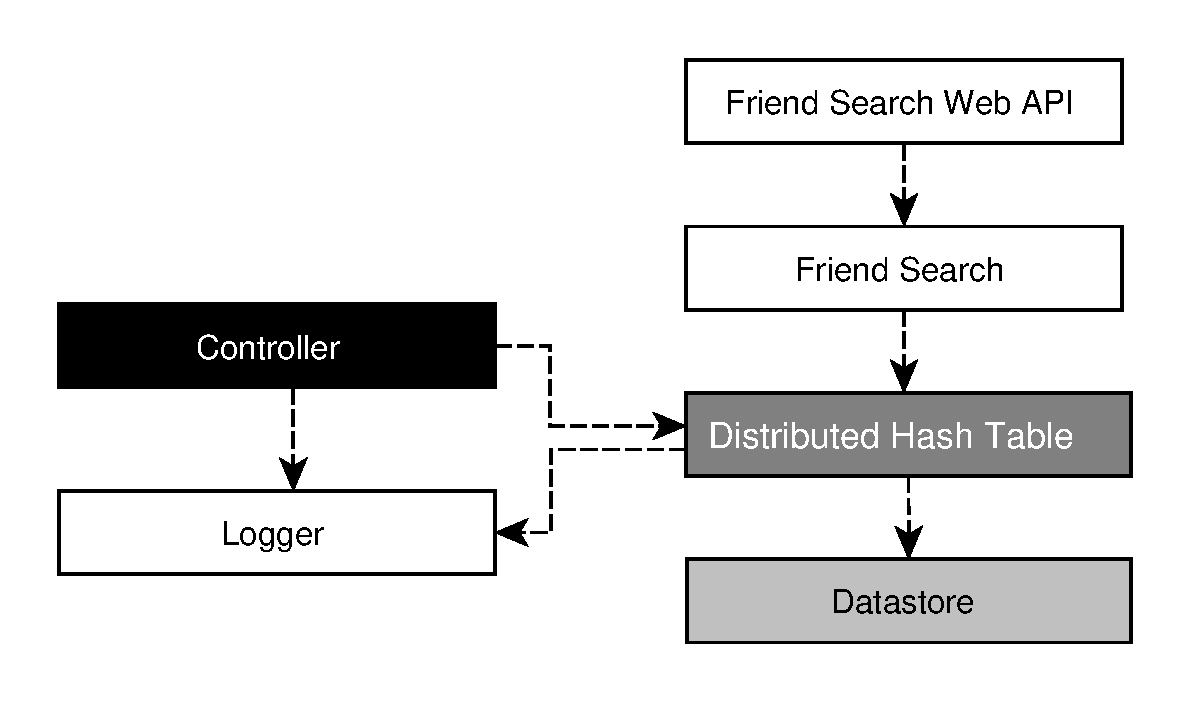
\includegraphics[width=0.9\linewidth]{illustrations/ComponentOverview.eps}
\caption{High level overview of the components of the search application. The arrows show the parts a component relies on.}
\label{figComponents}
\end{center}
\end{figure}

The arrows in figure \ref{figComponents} show which parts a component relies on to provide services for it. The Friend Search Web API exposes the HTTP API to the world and in turn uses the Friend Search server for resolving search queries into link records and then profile records that can be displayed to the end user. The Friend Search server uses the Distributed Hash Tables for finding the records, and the Distributed Hash Tables have local data stores that store the data items the particular Distributed Hash Table nodes are responsible for.

The controller is the component that interacts directly with the central control hub and starts and stops Distributed Hash Table nodes. It also regulates whether Pastry or Chord nodes should be run.

During experimental runs, the controller is also the component that issues requests to the locally run Distributed Hash Tables.

While a logger would certainly be included in the final release of the search engine, the one currently implemented would not be included as it is specific to the experimental setup.

\subsection{Third party code}
% Which components are not developed by me?
The Friend Search Web API in figure \ref{figComponents} uses an Erlang library called Webmachine for correctly handling HTTP requests. Webmachine in turn relies on another Erlang library called Mochiweb which the Friend Search Web API also uses in order to serialize the search results into JSON for consumption by the clients.

\section{Distributed Hash Tables}
Distributed Hash Tables are nothing but key-value stores where the data is stored across an array of hosts --- yet I am implementing two of them. The reason is that Chord and Pastry differ quite significantly in the way they approach finding out on which nodes data-items are stored. Not only do they differ in the way they organize and store their routing information, but unlike Chord, Pastry uses a proximity heuristic to favour nodes geographically closer to itself when routing. These differences in routing directly translate into differences in performance as is discussed in the evaluation chapter.

My implementation used a bag approach where I allow multiple items to be stored under the same key. This is necessary to avoid link records with common keys replacing each other.

The Chord key-space is an integer key-space ranging from 0 up to $2^{160} - 1$. It wraps around such that $2^{160} - 1$ immediately precedes 0. It can be useful to think of the key-space as circular. Just like the Chord key-space the Pastry key-space is also an integer key-space. While the Pastry paper \cite{pastry} suggests using keys in the range of 0 up to $2^{128} - 1$, I decided to let the Pastry key-space range from 0 to $2^{160} - 1$ just like for Chord, to increase code reuse between my Chord and Pastry implementations.
128-bit keys, as suggested in the Pastry paper \cite{pastry}, are easier to store efficiently in memory on 64-bit machines, which are common today, but other than that there is no evidence in the paper indicating that the performance of the Pastry algorithm should be any worse using 160-bit rather than 128-bit keys.

All data in Chord and Pastry is stored under 160-bit keys. The Chord and Pastry nodes themselves are also associated with keys in the same key-space as the data items. I use a hash of the hosts public IP-address and the port number a given node is listening to in order to determine a Distributed Hash Table node's key.

A node's key plays a significant role in splitting up the key-space between the nodes in the Distributed Hash Table. For this reason it is important that the keys are evenly distributed in the key-space so the amount of key-space each node is responsible for is roughly the same.

A Chord node is responsible for all the keys greater than the key of the node's predecessor and smaller or equal than the node's own key. In figure \ref{figKeyspaceChord}, the green node is responsible for the part of the key-space circle that is coloured green, the node coloured red for the part of the key-space coloured red, and likewise the yellow nodes for the part of the key-space that is yellow in colour.
A Pastry node, on the other hand, is responsible for all key-values that are numerically closer to the node's own key than to the key of the nodes on either side of it in the key-space. In figure \ref{figKeyspacePastry}, you can see how the green and the red node are each responsible for half the key-space between them. Likewise, the red and the yellow node are each responsible for half of the key-space between their respective key-values.

\begin{figure}[!htb]
\begin{center}
	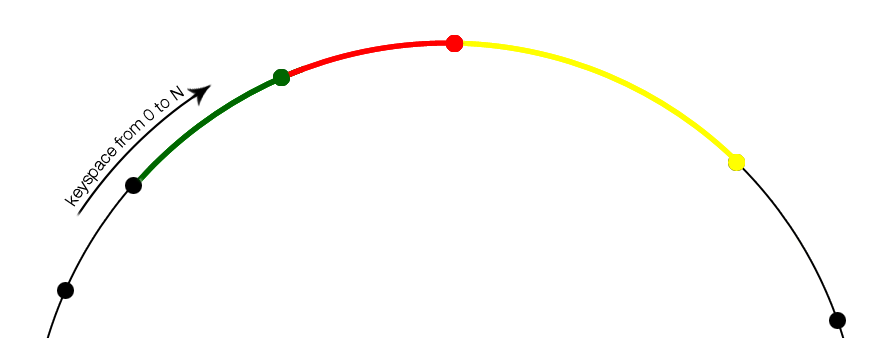
\includegraphics[width=0.9\linewidth]{illustrations/ChordKeySpace.png}
  \caption{Illustration of how the keyspace is divided between Chord nodes.}
  \label{figKeyspaceChord}
\end{center}
\end{figure}

\begin{figure}[!htb]
\begin{center}
	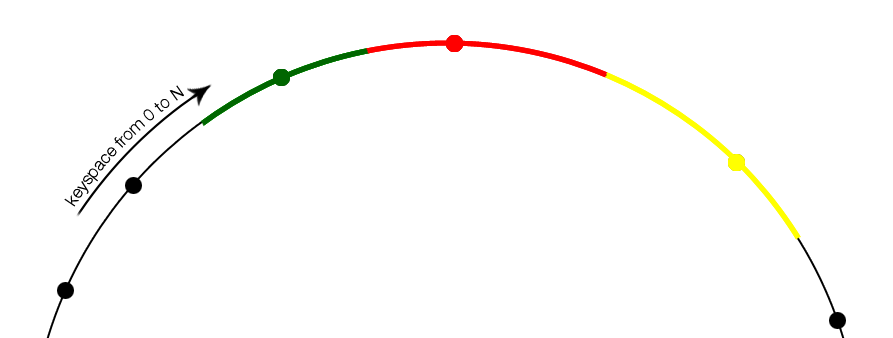
\includegraphics[width=0.9\linewidth]{illustrations/PastryKeySpace.png}
  \caption{Illustration of how the keyspace is divided between Pastry nodes.}
  \label{figKeyspacePastry}
\end{center}
\end{figure}

Just like in regular hash tables, the performance is best if a good hashing function is used to generate keys so that the keys are uniformly distributed in the key-space. This minimizes collisions but, in the case of Distributed Hash Tables, also ensures that the nodes in the network store approximately equal amount of data. The traffic distribution in the network depends on the distribution of the keys being requested. This might not be as uniform, but if the keys requested are spread out in the key-space, the traffic, much like the data, will also be spread out between the nodes in the network.

In order to be able to use Chord or Pastry interchangeably I specified a minimalistic API they should implement. It has functions for setting and getting values and for starting and stopping Distributed Hash Table nodes.

\subsection{Data structures}
To better understand how the routing algorithms work, let us first look at the data structures used by Chord and Pastry for storing the routing information.

\subsubsection{Chord's routing state}
\label{sec:chordRoutingState}
The Chord routing table contains an array of what, in chord jargon, are called fingers.
Each finger contains a start value which depends on the finger's position in the array and the node's own id, as well as a reference to the first node in the Chord network with a key greater than that start value.
Additionally, each finger contains an interval consisting of its own start value and the start value of the next finger.
The node stored in the $ 0^{th} $ entry of the finger array is the node's successor node, the node in the subsequent entry represents a node slightly further away, and the entries following after that likewise contain nodes with increasing key-space distance.
The routing table stores a total of 160 entries, one for each bit in the key.

Table \ref{tableChordRoutingTable} shows the Chord routing table and how each finger entry is calculated. It is taken from the Chord paper \cite{chord}. The values n, m and k are the node key, number of bits used for the key and index into the finger table array, respectively. 
The $ k^{th} $ finger entry has a start value that is half of the key-space greater than the node's own key-value, the $ k-1^{th} $ entry a node quarter of the key-space further away, and so on until the nodes immediately preceding the node are found.
This construction allows nodes to quickly close in on any given key-value by contacting another node which itself is at most half the key-space away from the key-value.
In this implementation m is always 160. Note that the array starts at 1 and not 0.

\begin{table}[h]
\caption{Values in the Chord routing table for a node with key n, using m-bit identifiers. k is an arbitrary array index into the finger array.}
\begin{center}
\begin{tabular}{ | l | l | }
  \hline                       
  Notation & Definition \\
  \hline  
  \hline  
  finger[k].start & $\left( n + 2^{k - 1} \right) mod \; 2^{m} , 1 \leq k \leq m $ \\
  \hline  
  \;.interval & $ \left[ finger[k].start, finger[k+1].start \right) $ \\
  \hline  
  \;.node & first node with key $ \geq n.finger[k].start $ \\
  \hline  
  predecessor & the previous node in the key-space \\
  \hline  
\end{tabular}
\end{center}
\label{tableChordRoutingTable}
\end{table}


\subsubsection{Pastry's routing state}
\label{sec:pastryRoutingState}
How does Pastry's routing table differ from that used by Chord?
A Pastry node maintains three separate data structures: a tuple called the leaf set containing a list of the nodes preceding and a list of nodes succeeding it in the key-space, a list of nodes called the neighbourhood set that are its neighbours in terms of the proximity heuristic used by Pastry, and a routing table. 
To make sense of the routing table let us first realize that while Chord looks at the key-space as an integer key-space in base 10, a Pastry node looks at the key-space as an integer key-space in an arbitrary base b.
The routing table is a list of lists of nodes that share an increasing number of digits in the key with the node itself. The first level entry in the routing table stores a list of nodes whose keys share no digits with the node. The second level entry stores nodes that share the first digit, and so on up until the last level entry where nodes share all but the very last digit.
In a sparsely populated network, most of the entries in the routing table will be left blank.
On the $ n^{th} $ level of the routing table, a node stores a list of nodes with keys that do not differ in any of the most significant digits up until the $ n^{th} $ key-digit.
A node will try to store nodes for all possible values of the $ n^{th} $ digit, so ideally a node that itself has an $ n^{th} $ digit of 0 will have entries for nodes with values 1 through b - 1 in their $ n^{th} $ digit key positions.

\mbox{}

Appendix \ref{sec:appendixErlangRoutingState} (page \pageref{sec:appendixErlangRoutingState}) shows how I translated the Chord and Pastry routing state into Erlang records.

\subsubsection{Example routing state}
The Chord and Pastry routing states can get quite abstract without a concrete example.
In figure \ref{figKeyspaceExample}, I show a reference 8-bit key-space with nodes drawn as dots. The green dot represents the node whose routing state we will inspect. Each node has two keys. The top one is the key as seen by Chord, and the bottom key is the key as it is seen by Pastry which, in this case, interprets the keys as numbers in base 4.

\begin{figure}[!htb]
\begin{center}
	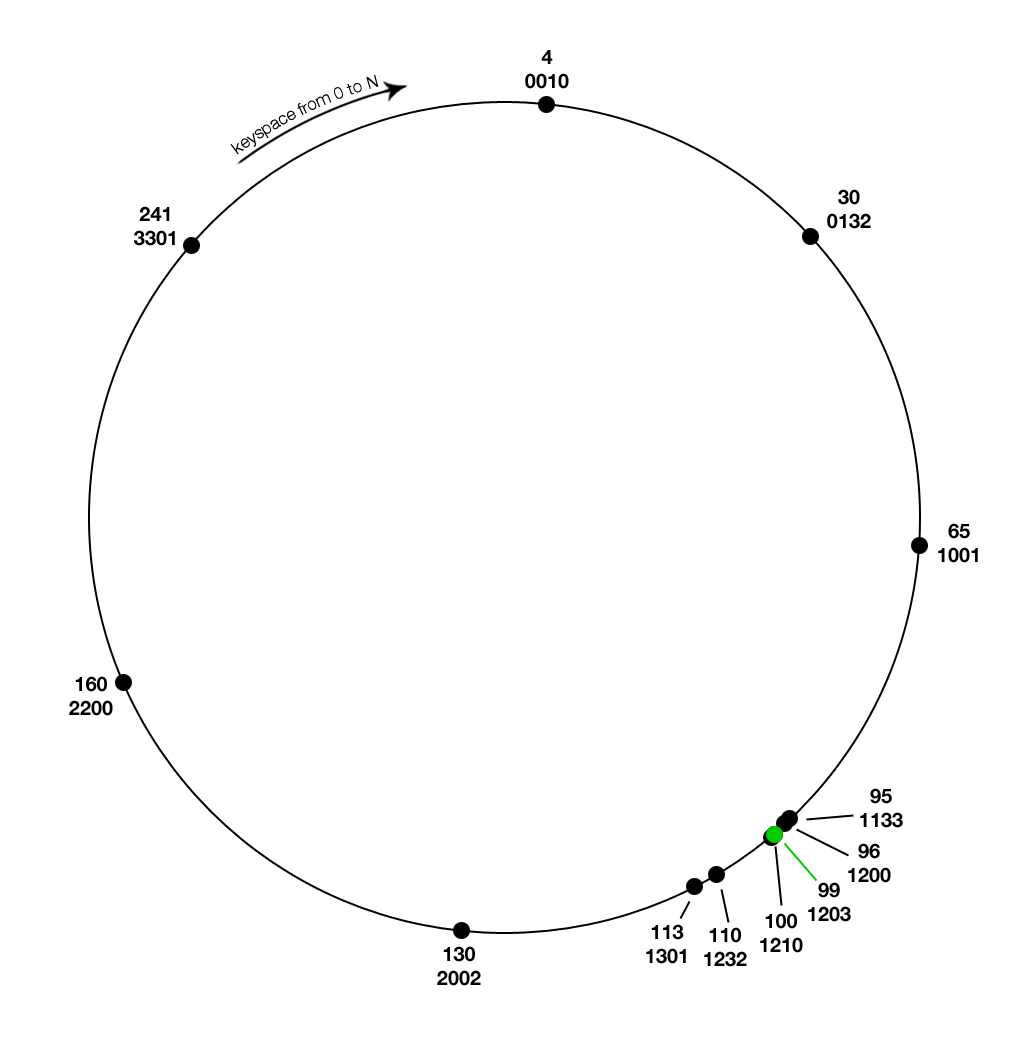
\includegraphics[width=0.9\linewidth]{illustrations/KeyspaceExample.png}
  \caption{Key-space with nodes. Each node has two keys. The top one is the key represented in base 10 as Chord sees it, and the bottom one in base 4 as seen by Pastry in this example.}
  \label{figKeyspaceExample}
\end{center}
\end{figure}

Table \ref{tableChordRoutingTableImpl} shows the routing state held by the Chord node with key 99, while table \ref{tablePastryRoutingTableImpl} shows the corresponding routing state for the same dot but as a Pastry node with key 1203.

\begin{table}[!htb]
\caption{Chord routing table for node 99 in figure \ref{figKeyspaceExample}.}
\begin{center}
\begin{tabular}{ | l | l | }
  \hline                       
  Field & Value \\
  \hline  
  \hline  
  % First finger
  finger[1].start & $ 99 + 2^{0} = 99 $ \\
  \hline  
  \;.interval & $ \left[ 99, 101 \right) $ \\
  \hline  
  \;.node & 100 \\
  \hline  
  % Second finger
  finger[2].start & $ 99 + 2^{1} = 101 $ \\
  \hline  
  \;.interval & $ \left[ 101, 103 \right) $ \\
  \hline  
  \;.node & 110 \\
  \hline  
  % Third finger
  finger[3].start & $ 99 + 2^{2} = 103 $ \\
  \hline  
  \;.interval & $ \left[ 103, 107 \right) $ \\
  \hline  
  \;.node & 110 \\
  \hline  
  % Fourth finger
  finger[4].start & $ 99 + 2^{3} = 107 $ \\
  \hline  
  \;.interval & $ \left[ 107, 115 \right) $ \\
  \hline  
  \;.node & 110 \\
  \hline  
  % Fifth finger
  finger[5].start & $ 99 + 2^{4} = 115 $ \\
  \hline  
  \;.interval & $ \left[ 115, 131 \right) $ \\
  \hline  
  \;.node & 130 \\
  \hline  
  % Sixth finger
  finger[6].start & $ 99 + 2^{5} = 131 $ \\
  \hline  
  \;.interval & $ \left[ 131, 163 \right) $ \\
  \hline  
  \;.node & 160 \\
  \hline  
  % Seventh finger
  finger[7].start & $ 99 + 2^{6} = 163 $ \\
  \hline  
  \;.interval & $ \left[ 163, 227 \right) $ \\
  \hline  
  \;.node & 241 \\
  \hline  
  % Eighth finger
  finger[8].start & $ 99 + 2^{7} = 227 $ \\
  \hline  
  \;.interval & $ \left[ 227, 99 \right) $ \\
  \hline
  \;.node & 241 \\
  \hline  
  predecessor & 96 \\
  \hline  
\end{tabular}
\end{center}
\label{tableChordRoutingTableImpl}
\end{table}

\begin{table}[!htb]
\caption{The Pastry routing state for Pastry node 1203 in figure \ref{figKeyspaceExample}. The emphasized digits in the routing table indicate at which digit the node keys differ from the node's own key.}
\begin{center}
\begin{tabular}{ | l | l | l | }
  \hline
  \multicolumn{3}{|c|}{Leaf set} \\ 
  \hline
  \hline                       
  Greater: & 1210 & 1232 \\
  \hline                       
  Smaller: & 1200 & 1133 \\
  \hline                       
\end{tabular}
\begin{tabular}{ | l | l | l | l | }
  \hline                       
  \multicolumn{4}{|c|}{Neighbourhood set} \\ 
  \hline
  \hline                       
  0010 & 1301 & 3301 & 1001 \\
  \hline                       
\end{tabular}
\begin{tabular}{ | l | l | l | l | }
  \hline                       
  \multicolumn{4}{|c|}{Routing table} \\ 
  \hline
  \hline                       
  \cellcolor{green} none & \emph{\textbf{0}}010 & \emph{\textbf{2}}200 & \emph{\textbf{3}}301 \\
  \hline                       
  \cellcolor{green} 1st & 1\emph{\textbf{0}}01 & 1\emph{\textbf{1}}33 & 1\emph{\textbf{3}}01 \\
  \hline                       
  \cellcolor{green} 2nd & 12\emph{\textbf{1}}0 & 12\emph{\textbf{3}}2 & \\
  \hline                       
  \cellcolor{green} 3rd & 120\emph{\textbf{0}} & & \\
  \hline                       
\end{tabular}
\end{center}
\label{tablePastryRoutingTableImpl}
\end{table}

\subsection{Routing}
%   What is different between Chord and Pastry?
%   How is routing done?
The routing algorithms for both Chord and Pastry are reasonably compact. I will give you an example of how the routing works before showing the pseudo-code from the Chord \cite{chord} and Pastry \cite{pastry} papers. Then, I show the corresponding Erlang implementations.

I have omitted supporting functions from the Erlang sample code that do not add to the understanding of the routing procedure in order to keep the source code listings concise.

\subsubsection{Routing in Chord}
We now review what happens when a Chord node wants to get the value of a key. Let us call the node that wants the value the requester, and the node that is responsible for the key the target node. I will use figure \ref{figRoutingChord} to illustrate the procedure. In the figure, the nodes with the names A, B, D and E are the nodes that directly participate in finding the target node F.
When the requester wants to get the value of a key, it starts by finding the node in its own routing table with a key that most closely precedes the key it wants to get the value of. In our example this is node B. It then asks that particular node if it knows about another node more closely preceding the target key. In this case node B knows about node D which has a key closer to the target key than what B itself does. The requester, node A, repeats the same question to node D and is returned node E. When node E is asked for the closest preceding node it returns itself, and it's successor F is asked for the contents of the key.

Notice how the Chord node A, the requester, is involved in all steps of the process of looking up which node stores the value of the key. This will become important in the evaluation section where we see what happens when we cannot connect to a node.

\begin{figure}[!htb]
\begin{center}
	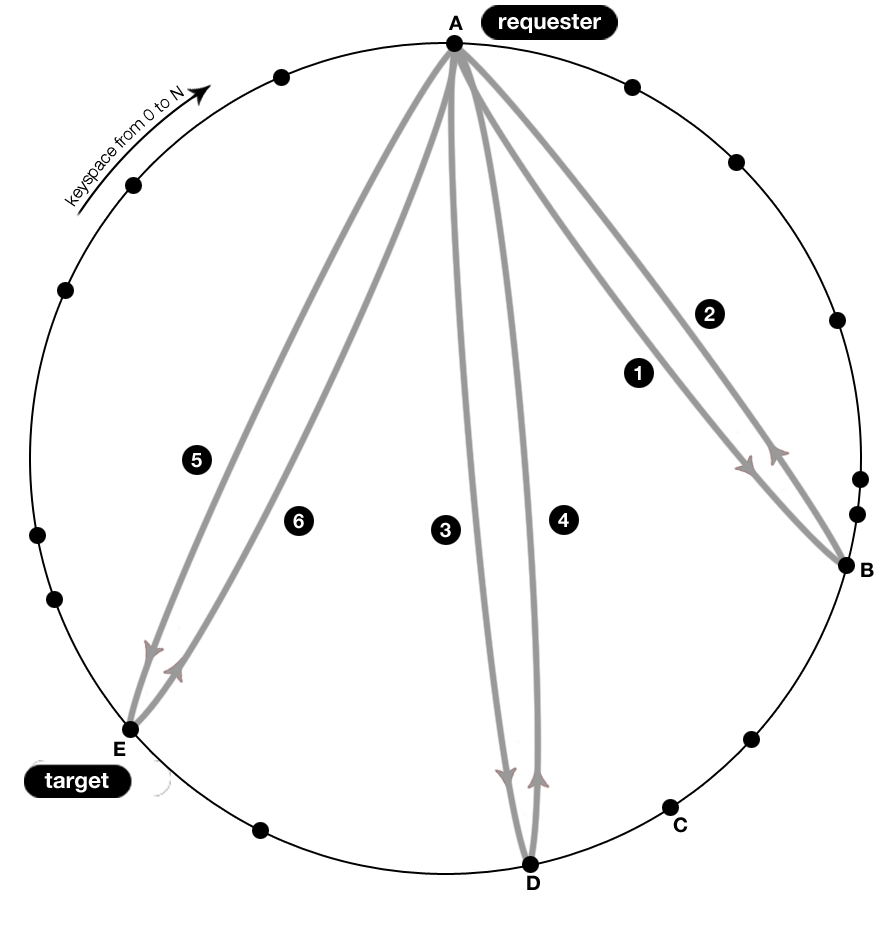
\includegraphics[width=0.9\linewidth]{illustrations/ChordRoutingSuccess.png}
  \caption{Chord's approach to routing.}
  \label{figRoutingChord}
\end{center}
\end{figure}

In the following code listings I will use the following conventions:
The syntax \verb=n.method_name()= indicates that the method with name \verb=method_name= is executed \emph{on} node \verb=n=. So when \verb=n'.method_name= is called on node \verb=n=, a remote procedure call to node \verb=n'= is being made.

Code listing \ref{listingChordPseudocode} shows the routing algorithm used by Chord as pseudo code. On line 10 in the code listing we see the method \verb=closest_preceding_finger= being invoked on node \verb=n'=. Using the routing example in figure \ref{figRoutingChord} \verb=n'= starts out as A, then changes to B etc.

\newpage

\lstinputlisting[label=listingChordPseudocode,caption=Chord routing pseudo code]{sourceCode/chord_pseudocode.txt}

Let us now take a quick look at each of the three methods from listing \ref{listingChordPseudocode} in turn and compare them to their Erlang equivalents.

The \verb=find_successor= method takes a key and finds its predecessor before returning the predecessor's successor.
Listing \ref{listingFindSuccessor} shows my Erlang implementation.
We see there is a very clear correspondence with the pseudo code implementation. First, the predecessor node is found on line 7 and its successor then returned on line 9.
What complicates the Erlang code slightly is that I wanted to implement the \verb=find_predecessor= while-loop using recursion. I therefore had to move the assignment on line 8 in the Chord pseudo code out to the \verb=find_successor= function.

\lstinputlisting[label=listingFindSuccessor,caption=Finding the successor of a key]{sourceCode/find_successor.erl}

In code listing \ref{listingFindPredecessor}, I show the Erlang equivalent of the Chord \verb=find_predecessor= pseudo code. 
In the pseudo code there are two remote procedure calls being done. One is to get a node's successor, and, only conditionally, one requests the node's closest preceding finger.
In my implementation, these two remote procedure calls have been made into one and for this reason this call has been moved to the very front of the function.
Notice how on line 11 in the Erlang implementation we use recursion rather than the while-loop used in the pseudo code. The equivalent of line 8 in the Chord pseudo code had to be moved out to the \verb=find_successor= function.

\lstinputlisting[label=listingFindPredecessor,caption=Finding the predecessor of a key]{sourceCode/find_predecessor.erl}

The procedure for finding the \verb=closest_preceding_finger= follows below. Unfortunately, it is slightly more complicated than the pseudo code equivalent. Since I am storing a list of successors for fault tolerance rather than a single successor, the case of the $ 0^{th} $ finger entry has to be handled separately. 
The bounds checking performed on line 16 in the Chord pseudo code was moved to a helper function called \verb=check_closest_preceding_finger= to avoid having to duplicate it in the \verb=closest_preceding_finger= function.
This function in turn makes a call back to \verb=closest_preceding_finger= if the finger entry is not a match.
The function in listing \ref{listingClosestPrecedingFinger} recursively looks at each finger in the routing table, checking if it is valid and returning the first one it finds that is.

\lstinputlisting[label=listingClosestPrecedingFinger,caption=Returns the node most closely preceding the key]{sourceCode/closest_preceding_finger.erl}

The bounds check is implemented in the helper function \verb=check_closest_preceding_finger= in listing \ref{listingCheckClosestPrecedingFinger}.

\lstinputlisting[label=listingCheckClosestPrecedingFinger,caption=Check if a finger is the closest known finger to a key. Returns the node most closely preceding the key]{sourceCode/check_closest_preceding_finger.erl}

\subsubsection{Routing in Pastry}
\label{sec:routingInPastry}
The Pastry approach differs quite significantly from Chord's approach to routing.
The most significant difference is that Chord nodes actively look for the node responsible for a key, and when that node is found, it contacts it in order to have it perform whatever task needs doing. Instead, Pastry performs message passing, where the message itself can contain information about whatever task the node wants done.
Also just like when sending mail through the postal system, the node loses visibility of the progress of the message as soon as it has been sent. This has the benefit of reducing the communication overhead and giving the sender time to perform other tasks or aid other nodes in their message sending while making it harder to notice if a message gets lost.

I illustrate the process in figure \ref{figRoutingPastry} where the requester of a key-value, node A, sends a \emph{lookup message} to the key it wants to look up. First, node A checks its own routing state for the node it knows about with a key closer to the target key than its own and sends its message to it. In this case, the node is node B. B in turn does the same and forwards the message to node D which in turn sends it on to the target node F. In the final step node F contacts the requester, node A, to let it know it is responsible for the value of the requested key. 

\begin{figure}[!htb]
\begin{center}
	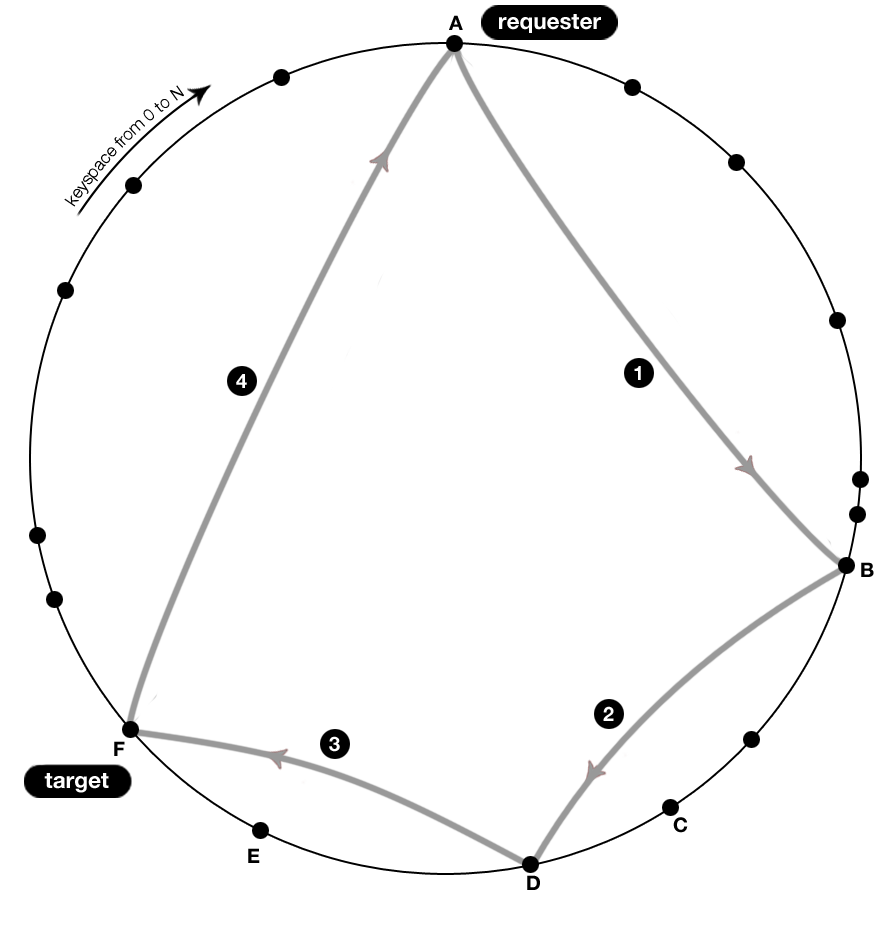
\includegraphics[width=0.9\linewidth]{illustrations/PastryRoutingSuccess.png}
  \caption{Pastry's approach to routing.}
  \label{figRoutingPastry}
\end{center}
\end{figure}

The following Pastry routing pseudo code is the pseudo code presented in the Pastry paper \cite{pastry}. 
It shows the method for routing a message for a target key k at a node with key n.

The Pastry routing approach works as follows: The node that is about to forward the message first checks if the recipient is in its leaf set. If it is, it delivers the message directly. The recipient could also be itself.
If there is no match in the leaf set, the routing table is used to find a node that shares an additional digit with the key with the message key compared to the node performing the routing. If there is no match in the routing table either, the Pastry node falls back to forwarding the message to any node it knows about that has a key numerically closer to the message key than the key the node itself has.

\lstinputlisting[label=listingPastryPseudocode,caption=Message routing pseudo code for Pastry]{sourceCode/pastry_pseudocode.txt}

The translation from Pastry pseudo code to Erlang implementation resembles the procedure used to implement the Chord algorithm in Erlang. It is described in more detail in Appendix \ref{sec:appendixErlangRoutingAlgorithm} on page \pageref{sec:appendixErlangRoutingAlgorithm}.

\subsection{Replication of data}
My implementations of Chord and Pastry both replicate data amongst their immediate neighbours for fault tolerance. While replication was only proposed as an extension in the Chord \cite{chord} and Pastry \cite{pastry} papers, I thought it worthwhile to add this functionality since my intended use was a search engine where I did not want data to become unavailable if an online social network provider decided to stop using my search network.

\section{Search server}
% Search server
The search server is what glues together the client facing HTTP API and the Distributed Hash Tables. It receives the search queries from the clients, converts them into appropriate keys that it can lookup in the Distributed Hash Tables, and resolves link records it gets returned to full profile records that can be shown as search results.

While the current implementation does basic ranking of results, prioritising what it predicts are better matches, it performs no caching of results which would significantly improve the performance.

\section{Central control hub}
% Hub control server
% Focus on testing and evaluation
The central control hub is an application that runs under a domain name known by all instances of the search engine application.
When the search engine application is started on a host, it registers itself with the control hub which in turn tells it how many nodes and of what Distributed Hash Table type should be run.

When new Distributed Hash Table nodes are started they also contact the control hub to get information about which other nodes they should try to connect to in order to join the Distributed Hash Table network.

The control hub is the only single point of failure in the system. If it becomes unavailable, no new search engine hosts can join because they cannot register and get information about which Distributed Hash Table type is being used. In addition, the existing hosts cannot start new Distributed Hash Table nodes because the nodes cannot contact the central control hub to get information about nodes they could use to join the Distributed Hash Table network. All hosts that are already registered remain active, and once a Distributed Hash Table node has started it runs fully independently of the central control hub application.
One could allow hosts to start new nodes by directly telling them about other known nodes they can connect to, but that functionality is currently not implemented.

The experiments used to evaluate the system are also initiated by the central control hub through a web interface (figure \ref{figHubApp}) that allows me to set the rate at which requests should be issued and the duration of the experiment. The requests themselves are issued individually by each host running the Distributed Hash Table nodes.

\begin{figure}[!htb]
\begin{center}
	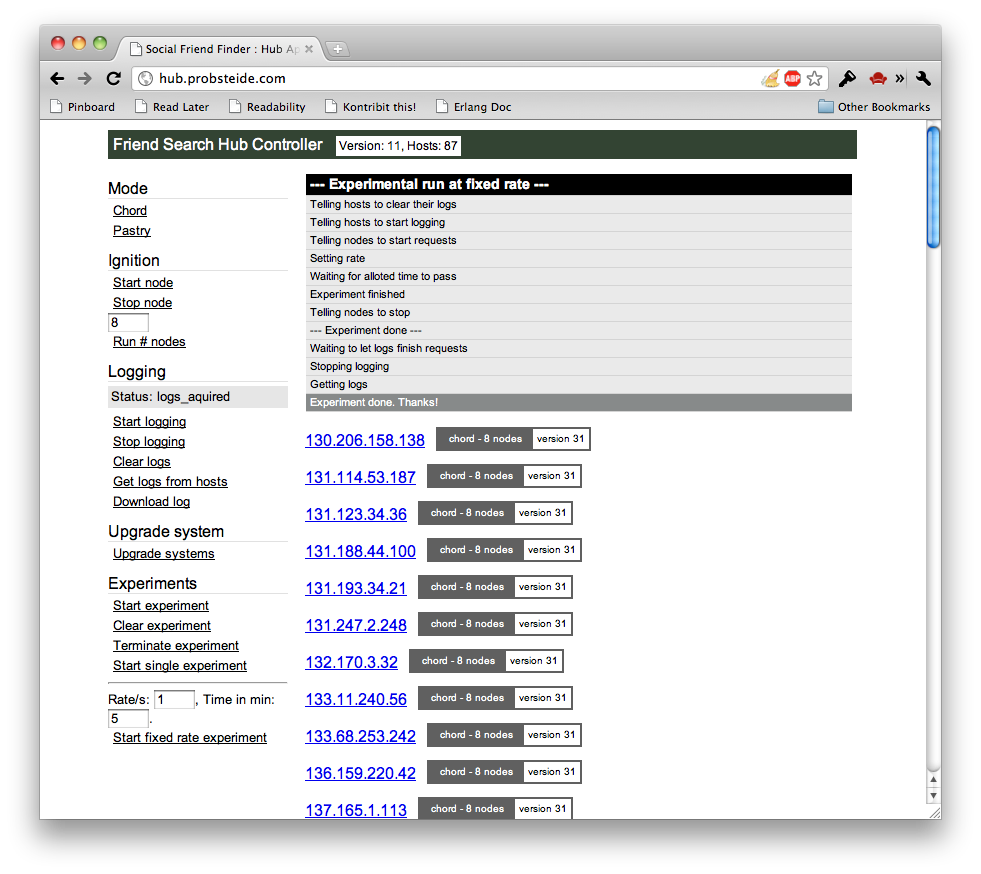
\includegraphics[width=0.9\linewidth]{illustrations/HubApp.png}
\caption{The Hub Application interface running on the central control hub. Shown here is the web interface that allows me to start and stop nodes, change between using Chord and Pastry, and start and stop experiments}
\label{figHubApp}
\end{center}
\end{figure}

Initially fully automated experiments were supported as outlined in my project proposal, but later, while evaluating my system, I removed the feature as it was impractical and didn't allow enough flexibility to run the experiments needed.

\section{Supervision for fault tolerance}
One of Erlang's main strengths is process supervision.
The supervision behaviour which is a part of the standard library makes it trivial to write processes supervising others. These processes are responsible for the lifetime behaviour of the processes they supervise, starting them when needed, restarting them if they terminate prematurely and stopping them when the application terminates. All supervisors with the exception of the root supervisor are themselves also supervised.

Process supervision is an important feature as it encourages designing minimal and isolated modules with individual life cycle control that can fail independently without bringing down the system. As failing modules are automatically restarted without impact on other components, one can easily build systems with high availability.
Another direct benefit also encouraged by Erlang and its designers is to write optimistic code handling what you as a designer think of as the optimal case, rather than practising defensive coding where you constantly have to check for malformed inputs. Malformed input, which would cause a process to crash, does not affect the availability of the system since the crashed process is automatically and immediately restarted. The direct benefit of this approach is that the code base becomes smaller and much easier to read and maintain.

Figure \ref{figSupervisionTree} shows the supervisors and the servers used in the main friend search application I developed.

\begin{figure}[!htb]
\begin{center}
	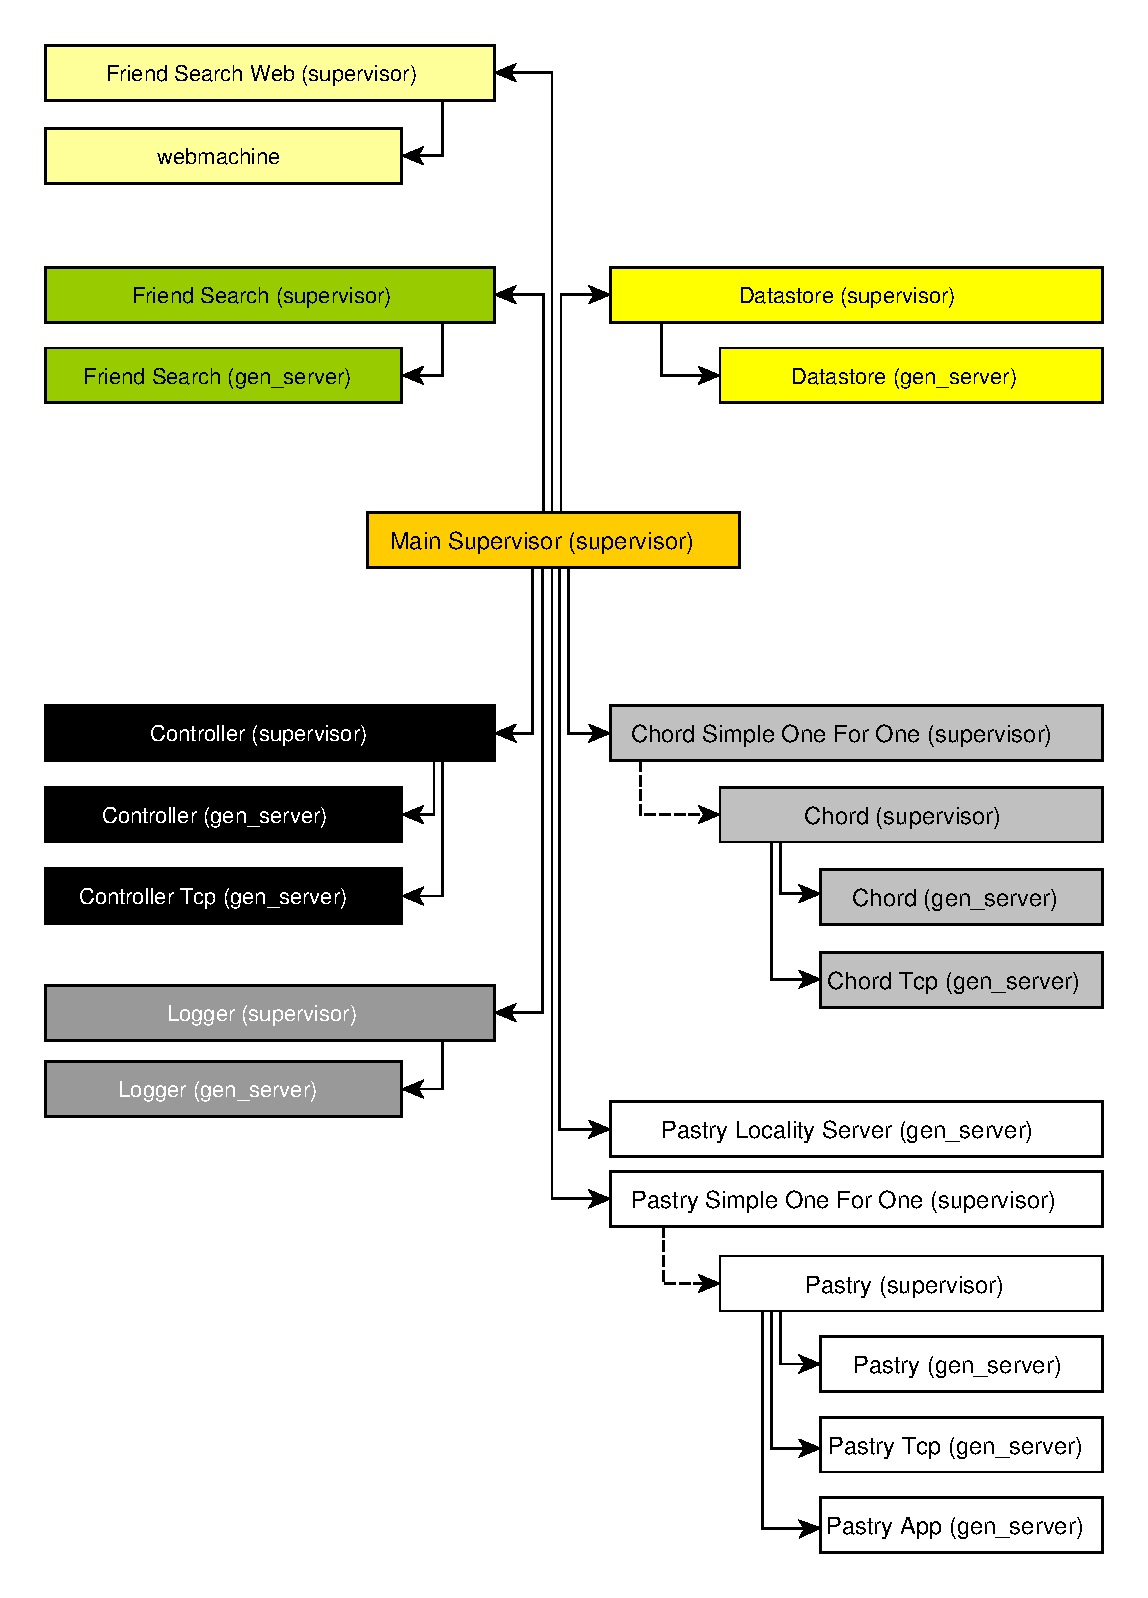
\includegraphics[width=0.9\linewidth]{illustrations/ClientSupervisionTree.eps}
  \caption{This figure shows the hierarchy of supervisors and the servers they supervise.}
  \label{figSupervisionTree}
\end{center}
\end{figure}

The root supervisor, represented by the box in the middle of figure \ref{figSupervisionTree}, supervises a wide range of other supervisors, all of which, with the exception of the Distributed Hash Table supervisors, supervise servers that are started at the same time as the application. 
The Chord and Pastry supervisors are a special kind of supervisor. They do not initially start any children, but can be signalled to start and maintain an arbitrary amount of children. This feature allows my system to, at runtime, dynamically adjust the number of Distributed Hash Table nodes that are run.


\section{Hot code reloading}
The Erlang virtual machine supports hot code reloading.
I built a code distribution service on top of this functionality that automatically updates the binary code of all running nodes whenever I pushed code changes to my code repository.

This greatly reduced the time it took to fix small bugs and experiment with changes after I had deployed my code to a large network of machines.

\mbox{}

In this chapter we have looked at how I developed my system. We looked at high level components and went into details of how routing differs between Chord and Pastry. We then looked at the other central components of my project, the central controlling hub and the search server.
Finally, we had a brief look at Erlang's supervisors and hot code reloading.
